The nuclear quantum many-body problem presents formidable challenges due to the strong spin–isospin dependence and intrinsically non-perturbative character of realistic nuclear interactions. In contrast to quantum chemistry, where the Coulomb interaction is known \emph{a priori} and provides a universal two-body potential, nuclear forces must be derived within the EFT framework. The construction of accurate two- and three-nucleon interactions with quantified uncertainties remains an active research frontier~\cite{epelbaum_modern_2009,machleidt_chiral_2011,ekstrom_what_2023}.

Recent advances in Bayesian parameter estimation and regulator optimization have further improved the consistency and predictive power of modern chiral EFT Hamiltonians.
The complexity of these interactions has motivated the development of a broad suite of \emph{ab initio} many-body approaches~\cite{hergert_guided_2020}. Single-particle basis methods, including the NCSM, CC theory, SCGF and the IMSRG, have achieved high-precision results across wide regions of the nuclear chart. Complementary stochastic formulations such as NLEFT have revealed striking signatures of clustering~\cite{shen_emergent_2023} and have advanced toward medium-mass nuclei, though their finite lattice spacing limits the resolution of short-range dynamics.
Continuum QMC methods~\cite{carlson_quantum_2015,lynn2019,gandolfi2020}, including GFMC~\cite{carlson_alpha_1988} and AFDMC~\cite{Schmidt:1999lik}, accurately capture nuclear dynamics from long to short distances, but their applicability across the nuclear chart remains restricted. GFMC scales exponentially with the mass number, while AFDMC suffers from a worsening sign problem for realistic chiral interactions~\cite{novario_trends_2023,martin_auxiliary_2023}.

Because this review focuses on neural quantum states (NQS) applied to continuum QMC, this section summarizes the local coordinate-space Hamiltonians derived from EFT that serve as inputs to both conventional QMC and NQS-based VMC calculations~\cite{gezerlis_local_2014}. We then discuss the principal scaling bottlenecks encountered by GFMC and AFDMC as the mass number increases, highlighting the aspects most relevant for constructing efficient NQS ans\"{a}tze. These considerations motivate the exploration of first-quantized NQS architectures that act directly on the continuous spatial coordinates and discrete spin–isospin degrees of freedom, offering a promising path toward extending the reach of continuum QMC methods beyond their traditional limits.


\subsection{Nuclear Hamiltonian}
\label{sub:hamiltonian}

To a remarkable extent, the properties of atomic nuclei and neutron-star matter can be described by point-like nucleons whose dynamics are governed by a nonrelativistic Hamiltonian  
\begin{align}
H_{LO} &= \sum_i \frac{\mathbf{p}_i^2}{2m_N} 
+ \sum_{i<j} v_{ij} 
+ \sum_{i<j<k} V_{ijk} \,,
\label{eq:ham}
\end{align}
where $\mathbf{p}_i$ is the three-momentum of the $i$-th nucleon, $m_N$ is its mass, and $v_{ij}$ and $V_{ijk}$ are the potentials describing nucleon-nucleon ($N\!N$) and three-nucleon ($3N$) interactions, respectively.

With the notable exception of Ref.~\cite{keeble_machine_2020}, and more recently Refs.~\cite{wen_neural-network_2025,yang_zemach_2025}, most applications of neural quantum states (NQS) to nuclear physics employ $N\!N$ and $3N$ potentials based on the premise that the momentum scales relevant for modeling the structure of atomic nuclei are much smaller than the pion mass, $m_\pi \simeq 140$ MeV. In this regime, pions can be integrated out, giving rise to pionless EFT~\cite{chen_nucleon-nucleon_1999,bedaque_effective_2002}, in which the charge-independent (CI) nuclear interactions consist solely of contact terms between two or more nucleons.
Pionless EFT provides a controlled and systematically improvable description of nuclear systems in the low-momentum regime, where short-range correlations and universal behavior dominate the structure of light nuclei and dilute nuclear matter. At the same time, its reduced operator complexity offers a natural setting for developing and benchmarking first-quantized NQS architectures, allowing one to isolate representational and optimization challenges before confronting the additional multiscale structure and strong tensor correlations induced by explicit pion exchange.



In this review, we focus on the leading-order (LO) pionless EFT expansion of Ref.~\cite{schiavilla_two-_2021}. The LO $N\!N$ interaction derived in that work is constrained to act only in even partial waves. In coordinate space, it is given by  
\begin{equation}
v_{LO}^{CI}(r_{ij}) = C_{01} C_1(r_{ij}) P_0^\sigma P_1^\tau 
                   + C_{10} C_0(r_{ij}) P_1^\sigma P_0^\tau ,
\label{eq:vNN_LO}
\end{equation}
where $r_{ij} = |{\bf r}_i - {\bf r}_j|$ and $P_{0,1}^\sigma$ ($P_{0,1}^\tau$) are the spin (isospin) projection operators for the nucleon pair $ij$ with total spin $S$ and isospin $T$ equal to 0 or 1:  
\begin{equation}
P_0^\sigma = \frac{1 - \sigma_{ij}}{4},\qquad
P_1^\sigma = \frac{3 + \sigma_{ij}}{4},\qquad
P_0^\tau   = \frac{1 - \tau_{ij}}{4},\qquad
P_1^\tau   = \frac{3 + \tau_{ij}}{4}\, .
\end{equation}
Here, $\sigma_{ij} = {\boldsymbol \sigma}_i \cdot {\boldsymbol \sigma}_j$ and $\tau_{ij} = {\boldsymbol \tau}_i \cdot {\boldsymbol \tau}_j$, with ${\boldsymbol \sigma}_i$ and ${\boldsymbol \tau}_i$ denoting the Pauli spin and isospin operators acting on nucleon $i$, respectively. In this implementation, the contact interactions are regularized using Gaussian cutoff functions,  
\begin{equation}
C_{\alpha}(r) = \frac{1}{\pi^{3/2} R_\alpha^3} \, e^{-(r / R_\alpha)^2} ,
\end{equation}
where $R_\alpha$ controls the range of the regulator.

\begin{figure}[!t]
    \centering
    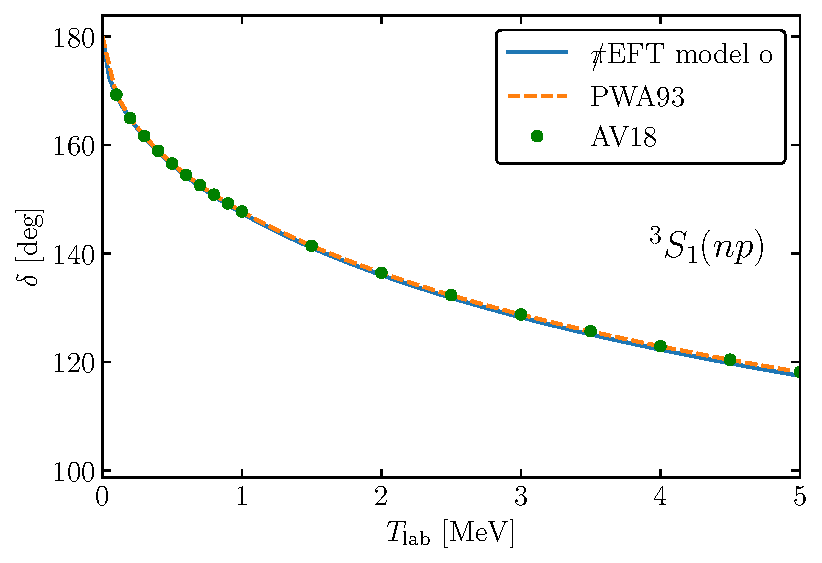
\includegraphics[width=0.49\linewidth]{figures/many_body_problem/phase_shifts_S1_T0_MT0.pdf}
    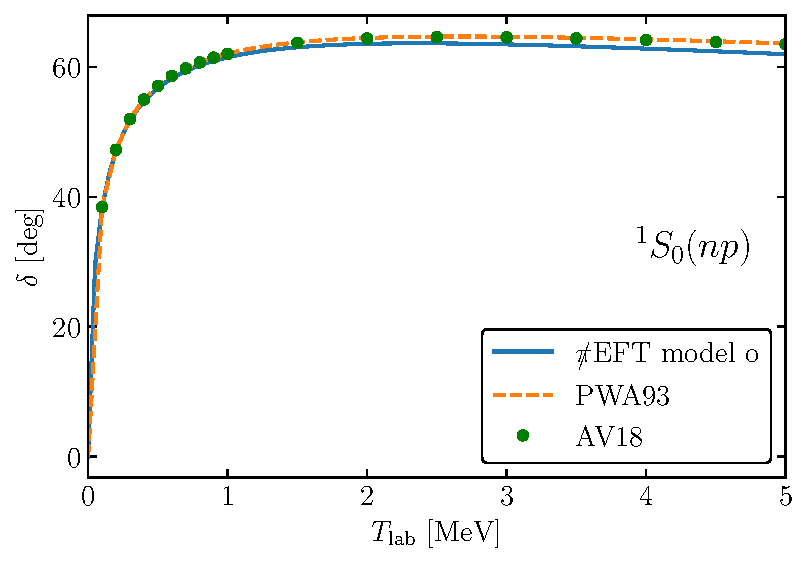
\includegraphics[width=0.49\linewidth]{figures/many_body_problem/phase_shifts_S0_T1_MT0.pdf}
\caption{Phase shifts in the $^3S_1$ and $^1S_0$ channels for $np$ scattering computed using the LO EFT Hamiltonian ``o'' of Ref.~\cite{schiavilla_two-_2021}, compared to the PWA93 analysis and results from the realistic Argonne v$_{18}$ potential~\cite{wiringa_accurate_1995}.}
 \label{fig:phases_np}
\end{figure}

\begin{figure}[!b]
    \centering
    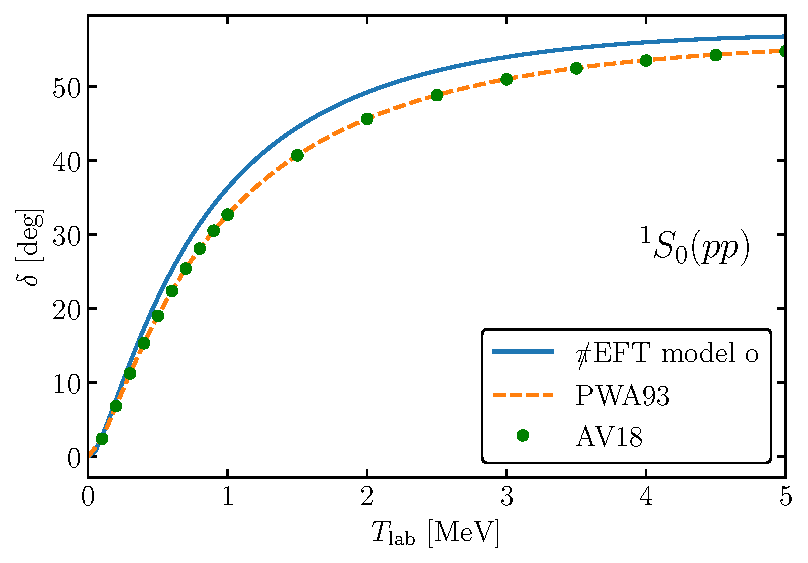
\includegraphics[width=0.49\linewidth]{figures/many_body_problem/phase_shifts_S0_T1_MT1.pdf}
    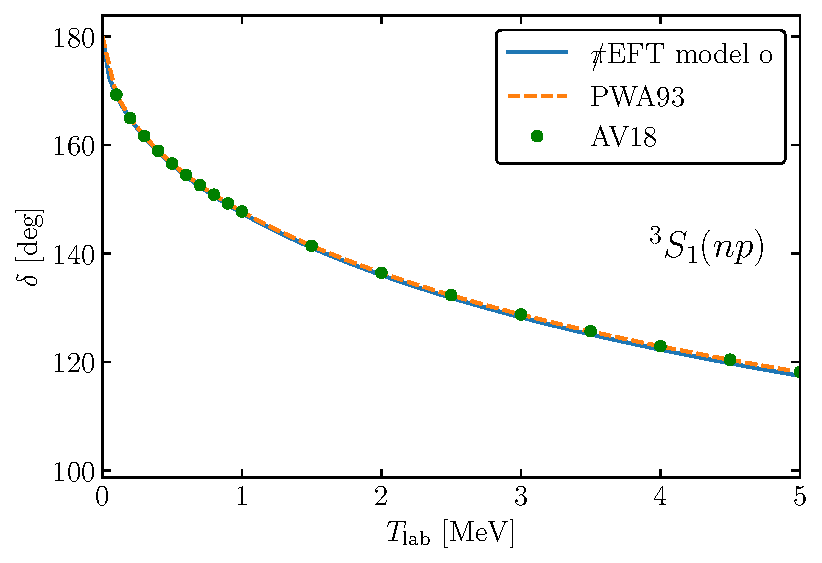
\includegraphics[width=0.49\linewidth]{figures/many_body_problem/phase_shifts_S1_T0_MT0.pdf}
\caption{Phase shifts in the $^1S_0$ channels for $pp$ and $nn$ scattering computed using the LO EFT Hamiltonian ``o'' of Ref.~\cite{schiavilla_two-_2021} compared to the PWA93 analysis and results from the realistic Argonne v$_{18}$ potential~\cite{wiringa_accurate_1995}..}
 \label{fig:phases_pp_nn}
\end{figure}

Most of the results presented in this review are obtained using model ``o'' of Ref.~\cite{schiavilla_two-_2021}, in which the cutoff radii $R_0 = 1.5459$ fm and $R_1 = 1.8304$ fm, as well as the low-energy constants $C_{01} = -5.27518671$ fm$^2$ and $C_{10} = -7.04040080$ fm$^2$, were adjusted to reproduce the neutron--proton scattering lengths and effective ranges in the singlet and triplet channels, as well as the deuteron binding energy. To demonstrate the performance of this interaction, Fig.~\ref{fig:phases_np} displays the phase shifts in the $^3S_1$ and $^1S_0$ channels for $np$ scattering. 

On the one hand, we observe excellent agreement with both the PWA93 analysis and those obtained from the highly realistic Argonne v$_{18}$ potential, extending up to $T_{\rm lab} = 5$ MeV.
On the other hand, the phase shifts of the model ``o'' in the $^1S_0$ channels for $pp$ and $nn$ scattering, displayed in Fig.~\ref{fig:phases_pp_nn}, exhibit some discrepancies compared to both the PWA93 analysis and those obtained from the realistic Argonne v$_{18}$ potential~\cite{wiringa_accurate_1995}. These differences can be attributed to the absence of a charge-dependent term in model ``o'', which enters at next-to-leading order (NLO) in the pionless EFT expansion. It has yet to be determined whether including these terms will stabilize $^6$He, $^8$Li, $^8$B, $^9$C, and $^{17}$F against breakup into smaller clusters, or if P-wave terms need to be incorporated into the nucleon-nucleon interaction~\cite{gattobigio_embedding_2019}.

The $N\!N$ potential of Eq.~\eqref{eq:vNN_LO} can be expressed compactly in the spin--isospin operator basis as  
\begin{align}
    v^{\rm CI}_{ij} = \sum_{p=1}^4 v^{p}(r_{ij}) O^p_{ij} \,,
    \label{eq:NN_op}
\end{align}
where $O^{p=1,4}_{ij} = \bigl( 1, \tau_{ij}, \sigma_{ij}, \sigma_{ij} \tau_{ij} \bigr)$, akin to the $v_4^\prime$ potential~\cite{wiringa_evolution_2002}. The explicit forms of the radial functions $v^p(r_{ij})$ are provided in Appendix~A of Ref.~\cite{schiavilla_two-_2021}, and their radial dependence is illustrated in Fig.~\ref{fig:v_NN}.


\begin{figure*}[!t]
\centering
  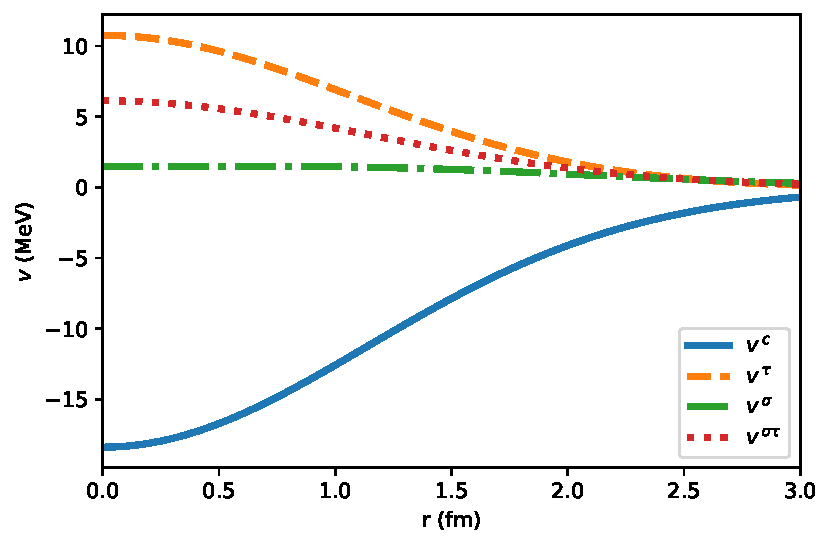
\includegraphics[width=0.6\textwidth]{figures/many_body_problem/v_NN.pdf}
\caption{Radial functions of the model ``o'' $N\!N$ potential at LO in the pionless EFT expansion, expressed in the spin--isospin basis.}
\label{fig:v_NN}
\end{figure*}

In addition to the CI component, the two-nucleon interaction includes an electromagnetic (EM) contribution, such that $v = v^{\rm EM} + v^{\rm CI}_{\rm LO}$. The full $v^{\rm EM}$ consists of one- and two-photon Coulomb terms, the Darwin-Foldy term, vacuum polarization, and magnetic moment interactions; see Ref.~\cite{wiringa_accurate_1995} for their explicit expressions. However, most NQS applications retain only the Coulomb repulsion between finite-size (rather than point-like) protons.  

In pionless EFT, solving systems with $A \geq 3$ using purely attractive LO $N\!N$ potentials leads to the so-called Thomas collapse~\cite{yang_we_2020} as the regulator is removed. This pathological behavior is avoided by promoting a contact $3N$ force to LO~\cite{bedaque_renormalization_1999}. In this review, we consider a regularized $3N$ potential of the form  
\begin{align}
    V_{ijk} = \frac{c_E}{f_\pi^4 \Lambda_\chi} \frac{(\hbar c)^6}{\pi^3 R_3^6} 
    \sum_{\rm cyc} e^{-(r_{ij}^2 + r_{jk}^2)/R_3^2} ,
    \label{eq:o_3NF}
\end{align}
where $\Lambda_\chi = 1$ GeV, $f_\pi = 92.4$ MeV is the pion decay constant, and $\sum_{\rm cyc}$ denotes cyclic permutations of the indices $i$, $j$, and $k$. The low-energy constant $c_E$ is fixed to reproduce the $^3$H binding energy, $B(^3$H$) = 8.475$ MeV, for a given value of the cutoff $R_3$.  The analysis of Ref.~\cite{schiavilla_two-_2021} shows that the choice $R_3 = 1.0$ fm and $c_E = 1.0786$ provides a satisfactory description of nuclear binding energies across a broad mass range, up to $^{90}$Zr. However, subsequent VMC–NQS calculations have indicated that this choice leads to overbinding in $^{16}$O and heavier nuclei. Increasing the cutoff to $R_3 = 1.1$ fm with $c_E = 1.2945$ largely resolves this issue~\cite{gnech_distilling_2024}, as the extended range of the $3N$ force introduces additional repulsion in heavier systems.

\begin{figure*}[!t]
\centering
  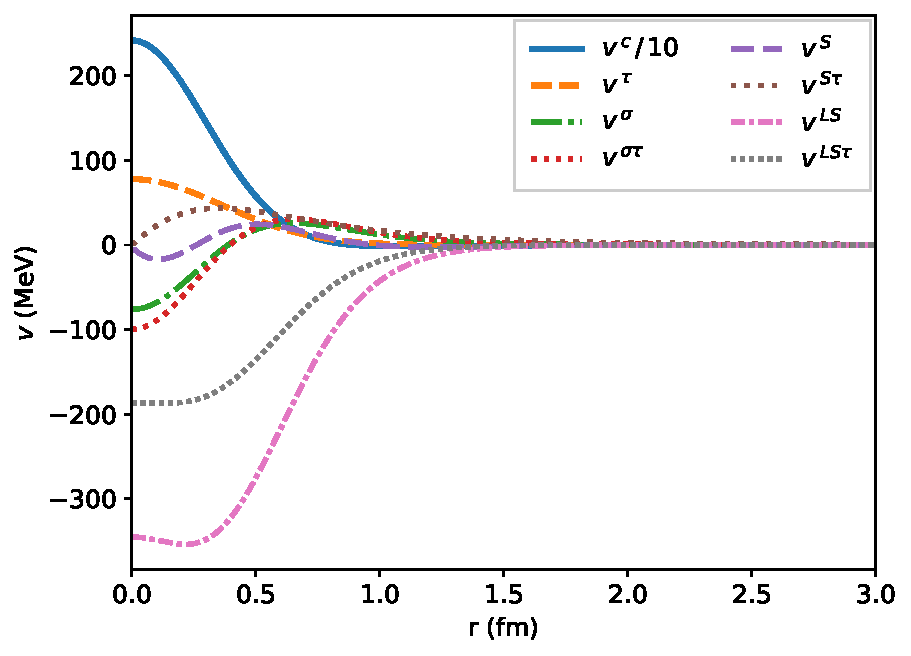
\includegraphics[width=0.6\textwidth]{figures/many_body_problem/AV8P.pdf}
\caption{Radial functions of the Argonne $v_8^\prime$ potential, expressed in the spin–isospin basis.}
\label{fig:av8p}
\end{figure*}


Very recent applications of nuclear NQS employ higher-resolution interactions, either phenomenological or derived within chiral EFT. In particular, Refs.~\cite{yang_chiral_2025,wen_neural-network_2025,yang_zemach_2025} use consistent $NN$ and $3N$ potentials derived at next-to-next-to-leading order (N$^2$LO) in the chiral EFT expansion that are local in coordinate space~\cite{gezerlis_quantum_2013,gezerlis_local_2014,lynn_chiral_2016}. Notably, the authors of Ref.~\cite{yang_chiral_2025} were also able to employ NQS with the phenomenological Argonne $v_8^\prime$ + Urbana IX Hamiltonian~\cite{pudliner_quantum_1995}, which features a strongly repulsive core at short distances.
The charge-independent (CI) part of both the Argonne $v_8^\prime$ interaction and the local N$^2$LO chiral EFT potentials can be written in operator form as
\begin{equation}
v_{ij} = \sum_{p=1}^{8} v^p(r_{ij}) O^p_{ij}\,,
\label{eq:vij_op_sum}
\end{equation}
where $r_{ij} = |{\bf r}_i - {\bf r}_j|$ is the interparticle distance.
For the local N$^2$LO chiral EFT potential, the sum is restricted to the first seven operators.
Compared to Eq.~\eqref{eq:NN_op}, the additional operators entering this expansion include the tensor and spin-orbit components, for a total of eight operators, where $O^{p=5,8}_{ij} = \bigl( S_{ij}, S_{ij}\, \tau_{ij}, \mathbf{L} \cdot \mathbf{S}, \mathbf{L} \cdot \mathbf{S}\, \tau_{ij} \bigr)$. 
The tensor operator is
\begin{equation}
S_{ij}= \frac{3}{r^2_{ij}}(\boldsymbol{\sigma}_i\cdot {\bf r}_{ij})(\boldsymbol{\sigma}_j \cdot{\bf r}_{ij})- \sigma_{ij}\, ,
\end{equation}
while the spin-orbit contribution is expressed in terms of the relative angular momentum $\mathbf{L}=\frac{1}{2 i} (\mathbf{r}_i -\mathbf{r}_j) \times (\nabla_i - \nabla_j)$ and the total spin $\mathbf{S}=\frac{1}{2}(\boldsymbol{\sigma}_i+\boldsymbol{\sigma}_j)$ of the pair. The radial functions of the Argonne $v_8^\prime$ potential are displayed in Fig.~\ref{fig:av8p}.  
In contrast to the model ``o'' interaction of Fig.~\ref{fig:v_NN}, the Argonne potential exhibits a very strong short-range repulsive core, exceeding 2~GeV (in the figure the central channel is divided by a factor of 5 for visibility). The sizable tensor and spin--orbit components, which extend to relatively large distances, are also clearly visible. This long-range behavior is a consequence of one-pion exchange. While the associated tensor interaction is singular at short distances in its bare form, scaling as $1/r^3$, this divergence is regularized in the Argonne interaction. The interaction nevertheless remains long-ranged in the Yukawa sense at large separations, decaying as $e^{-m_\pi r}/r$ up to polynomial factors, and provides the dominant source of tensor correlations at intermediate distances in nuclei. Note that the Coulomb interaction, which is the longest-ranged component of the nuclear Hamiltonian, decays as $1/r$ but is comparatively weak and acts only between protons. %This long-range behavior is a consequence of one-pion exchange, whose tensor part falls off only as $e^{-m_\pi r}/r^3$, making it the dominant source of intermediate- and long-range correlations in nuclei.

The earliest example of a $3N$ force dates back to the Fujita--Miyazawa interaction, whose main contributions arise from the virtual excitation of a $\Delta(1232)$ resonance in processes involving three interacting nucleons~\cite{fujita_pion_1957}. This term is included in both chiral EFT and in the Urbana IX potential~\cite{pudliner_quantum_1995} and reads 
\begin{equation}
V_{ijk}^\Delta = V_{ijk}^{\Delta,a} + V_{ijk}^{\Delta,c}\, .
\end{equation}
The ``anticommutator'' and ``commutator'' contributions are  
\begin{equation}
V_{ijk}^{\Delta,a} = \sum_{\rm cyc} 
A_{2\pi}\,\{X_{ij}^\pi, X_{jk}^\pi\}\,\{\tau_{ij}, \tau_{jk}\} \quad , \quad 
V_{ijk}^{\Delta,c} = \sum_{\rm cyc} 
C_{2\pi}\,[X_{ij}^\pi, X_{jk}^\pi]\,[\tau_{ij}, \tau_{jk}]\,,
\end{equation}
where $\sum_{\rm cyc}$ denotes a sum over the three cyclic permutations of the nucleons $i,j,k$.  
The operator $X_{ij}^\pi$ is defined as 
\begin{equation}
X_{ij}^\pi = T(r_{ij})\, S_{ij} + Y(r_{ij})\,\sigma_{ij}\,,
\end{equation}
where the radial Yukawa and tensor functions, $Y(r)$ and $T(r)$, are defined consistently with those appearing in the corresponding $NN$ interaction~\cite{wiringa_accurate_1995,pudliner_quantum_1997}.

Generally, a three-body potential composed only of $V_{ijk}^\Delta$ does not reproduce the empirical saturation density of isospin-symmetric nucleonic matter~\cite{lagaris_variational_1981}; a repulsive three-body contribution must be included,
\begin{equation}
V^{R}_{ijk} = A_R \sum_{\rm cyc} T^2(r_{ij})\, T^2(r_{jk}) \,.
\end{equation}
The constants $A_{2\pi}$ and $A_R$ entering the Urbana IX model are determined by fitting the binding energy of ${}^3$H and the saturation density of isospin-symmetric nucleonic matter, $\rho_0 = 0.16~\mathrm{fm}^{-3}$~\cite{Akmal:1998cf}.  
Chiral EFT interactions likewise include a short-range three-body operator proportional to the low-energy constant $c_E$. This contribution may be purely scalar or contain isospin dependence, although the latter appears to be incompatible with astrophysical constraints.

In addition to the terms above, chiral EFT three-body forces at N$^2$LO contain a one-pion-exchange (OPE) three-body component proportional to the low-energy constant $c_D$, as well as a second short-range contact proportional to $c_E$. The OPE three-body structure is also included in the phenomenological Illinois-7 force~\cite{pieper_illinois_2008}. For detailed discussions of these terms, we refer the reader to Refs.~\cite{lynn_quantum_2017}, while Ref.~\cite{lovato_comparative_2012} provides a comprehensive comparison between local phenomenological and chiral EFT interactions.


    
\subsection{Progress and challenges of quantum Monte Carlo methods}
\label{sub:qmc_methods}


The Hamiltonians discussed in the previous section are the main input to \emph{ab initio} many-body methods that, within controlled approximations, solve the nuclear Schr\"odinger equation
\begin{equation}
H |\Psi_n\rangle = E_n |\Psi_n\rangle\,,
\end{equation}
where $|\Psi_n\rangle$ denotes the $n$th eigenstate and $E_n$ its associated eigenvalue.
Several stochastic many-body frameworks have been developed to address this problem. 
Two broad and complementary approaches are lattice formulations based on path-integral methods and continuum quantum Monte Carlo techniques.

Nuclear lattice effective field theory (NLEFT)~\cite{epelbaum_ab_2011,lee_lattice_2025}, aided by notable algorithmic advances~\cite{sarkar_floating_2023}, has expanded its reach to medium-mass nuclei~\cite{elhatisari_wavefunction_2024}, provided compelling evidence for $\alpha$ clustering~\cite{shen_emergent_2023}, and explored nuclear and neutron matter at finite temperature~\cite{Ren:2023ued,ma_structure_2024}. 
However, NLEFT continues to face limitations arising from the fermion sign problem and the rapidly growing computational cost associated with fine lattice spacings, which constrain its ability to resolve short-range dynamics unless simplified interactions are used.

Continuum QMC methods~\cite{carlson_quantum_2015,gandolfi2020}, originally developed in condensed-matter physics and later adapted to nuclear systems, operate directly in coordinate space. 
The variational Monte Carlo (VMC) method optimizes a parametrized trial state to capture the most important correlations and enforce the correct asymptotic behavior, thereby accurately describing long-range dynamics and $\alpha$ clustering. 
Building on VMC, Green’s function Monte Carlo (GFMC)~\cite{carlson_greens_1987,carlson_alpha_1988} projects the variational state in imaginary time toward exact eigenstates, while auxiliary-field diffusion Monte Carlo (AFDMC)~\cite{Schmidt:1999lik} employs Hubbard--Stratonovich auxiliary fields to sample spin--isospin operators and access larger systems.  
These continuum approaches model nuclear dynamics across long, intermediate, and short distances and can accommodate ``stiff'' interactions with high-momentum components.  
Recent applications include ground-state properties~\cite{piarulli_light-nuclei_2018}, inclusive electron- and neutrino-scattering~\cite{lovato_ab_2020,andreoli_quantum_2024}, and a variety of electroweak observables such as electromagnetic moments and form factors, low-energy transitions and $\beta$ decays, and muon-capture processes~\cite{king_ab_2023,chambers-wall_quantum_2024}.



In this review, we focus primarily on the VMC method, first outlining the computational challenges of conventional variational states. VMC relies on the Rayleigh–Ritz variational principle
\begin{equation}
\frac{\langle \Psi_V(\params) \, | \, H \, |\,  \Psi_V(\params)\rangle}{\langle \Psi_V(\params) \, | \, \Psi_V(\params)\rangle} \equiv E_V(\params) \geq E_0
\label{eq:variational}
\end{equation}
to determine the optimal set of parameters $\params$ defining the variational state $\Psi_V$. For the nuclear many-body problem, it is customary to assume that the trial state factorizes into long- and short-range components,
\begin{equation}
\Psi_V(R,S) \equiv \langle  R,S \, |\Psi_V\rangle = \langle R S \, | \left(1 + \sum_{i<j<k} F_{ijk}\right)
\left(\mathcal{S}\prod_{i<j} F_{ij}\right) | \Phi \rangle\,,
\label{eq:variational_product}
\end{equation}
where $F_{ij}$ and $F_{ijk}$ are two- and three-body correlation operators, respectively. The symbol $\mathcal{S}$ denotes a symmetrized product over nucleon pairs, since—in general, owing to their spin--isospin dependence—the $F_{ij}$ need not commute. The symbol $R$ denotes the spatial coordinates of all nucleons, $(\mathbf{r}_1, \ \dots \ , \ \mathbf{r}_A )$, while $S$ stands for the spin--isospin degrees of freedom, to be discussed in detail below. 

The long-range antisymmetric part $\Phi$ is commonly expressed as a linear combination of a few Slater determinants built from single-particle orbitals appropriate to the system of interest. For homogeneous matter, the orbitals are usually plane waves and may include pairing correlations~\cite{gandolfi2009a}. For atomic nuclei, the single-particle orbitals are generally taken in the $ls$- or $jj$-coupling schemes and combined to yield the desired total angular momentum $J$ and parity $P$ of the nucleus~\cite{pudliner_quantum_1997}. Importantly, VMC calculations can explicitly incorporate the strong $\alpha$-cluster structure of light nuclei: the wave function of $p$-shell systems is constructed as a sum of independent-particle components, each with four nucleons in an $\alpha$-like core and the remaining $(A-4)$ nucleons occupying $p$-shell orbitals~\cite{pieper_quantum_2002}.

The spin--isospin structure of the two-body correlation operator mirrors that of the $NN$ potential and is written as
\begin{equation}
F_{ij} = \sum_{p=1}^{6} f^{p}(r_{ij}) O^{p}_{ij} .
\end{equation}
Spin-orbit correlations, corresponding to $p=7$, $8$, may also be included, but are often neglected due to the significant computational cost and the relatively small gain in variational energy~\cite{lonardoni_variational_2017}. The optimal radial functions $f^{p}(r)$ are typically obtained by minimizing the two-body cluster contribution to the ground-state energy, subject to the correct asymptotic behavior~\cite{lomnitz-adler_monte_1981}.
Appropriate three-body correlation form factors have been derived within perturbation theory, as discussed in Ref.~\cite{carlson_quantum_2015},
\begin{equation}
F_{ijk} = \sum_x \epsilon_x V_{ijk}^x(\tilde r_{ij}, \tilde r_{ik}, \tilde r_{jk}) ,
\label{eq:three_body_corr}
\end{equation}
where $\tilde r = y_x r$, with $y_x$ a variational scaling parameter and $\epsilon_x$ a small (negative) strength parameter, both optimized variationally. The superscript $x$ labels the different components of the three-nucleon interaction (e.g., $\Delta$, $R$).


Both the VMC and GFMC methods employ an explicit many-body basis for the
spin--isospin sector of the Hilbert space. A generic basis state can be written as $|S\rangle \equiv |\chi_{i_s}\rangle \otimes |\chi_{i_t}\rangle, $
where the indices $i_s$ and $i_t$ enumerate the many-body spin and isospin basis states, respectively. The $2^A$ spin basis states can be written as
\begin{align}
|\chi_1\rangle &= |\downarrow_1, \downarrow_2,\dots,\downarrow_A\rangle \nonumber, \\
|\chi_2\rangle &= |\uparrow_1, \downarrow_2,\dots,\downarrow_A\rangle \nonumber, \\
& \  \vdots \nonumber\\
|\chi_{n_s}\rangle &= |\uparrow_1, \uparrow_2,\dots,\uparrow_A\rangle\,,
\end{align}
with $n_s = 2^A$. The corresponding isospin states $|\chi_{i_t}\rangle$ are
obtained by replacing $\downarrow$ with $n$ and $\uparrow$ with $p$.
For fixed proton number $Z$ (charge conservation), the dimension of the isospin basis is $\binom{A}{Z}$.
Figure~\ref{fig:gfmc_scaling} shows the spin--isospin Hilbert-space dimension for nuclei treated with GFMC to date. Data shown includes $^{13}$C, currently being computed on ALCF’s Aurora supercomputer, and $^{16}$C, anticipated to be within reach of the next generation of leadership-class machines.

\begin{figure}[!t]
    \centering
    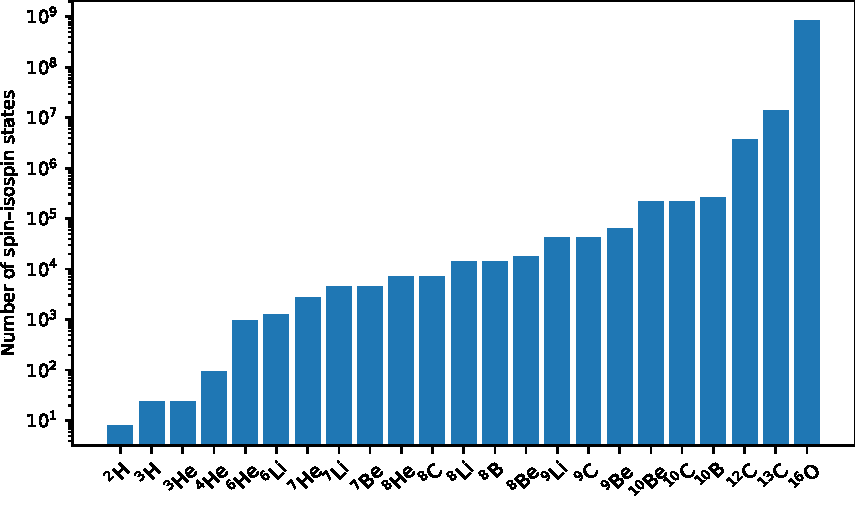
\includegraphics[width=0.8\linewidth]{figures/many_body_problem/spin_isospin_states.pdf}
\caption{Number of many-body spin--isospin states, $2^A \binom{A}{Z}$, relevant to VMC and GFMC calculations for selected light nuclei.\label{fig:gfmc_scaling}}
\end{figure}


The symmetrized product of pair correlation operators is evaluated by successive operations
for each pair, sampling their ordering. As an example, consider the application of the
operators $\sigma_{12} \sigma_{13} \sigma_{23}$ on the three-body spin state $|\uparrow_1, \downarrow_2, \downarrow_3\rangle$. Noting that $\sigma_{ij} = 2P^\sigma_{ij} - 1$, where $2P^\sigma_{ij}$ exchanges the spin of particles $i$ and $j$, we obtain:
\begin{align}
\sigma_{12}\, \sigma_{13}\, \sigma_{23} |\uparrow_1, \uparrow_2, \downarrow_3\rangle & = \sigma_{12}\, \sigma_{13} ( 2 |\uparrow_1, \downarrow_2, \uparrow_3\rangle - |\uparrow_1, \uparrow_2, \downarrow_3\rangle) \nonumber \\
& = \sigma_{12}\, ( 2 |\uparrow_1, \downarrow_2, \uparrow_3\rangle - 2 |\downarrow_1, \uparrow_2, \uparrow_3\rangle + |\uparrow_1, \uparrow_2, \downarrow_3\rangle) \nonumber \\
& = 4 |\downarrow_1, \uparrow_2, \uparrow_3\rangle - 6 |\uparrow_1, \downarrow_2, \uparrow_3\rangle - 2 |\downarrow_1, \uparrow_2, \uparrow_3\rangle + |\uparrow_1, \uparrow_2, \downarrow_3\rangle) \,.
\end{align}
Hence, even starting from a single spin state, the action of the correlation operator generates four of them (even more are generated by the tensor correlations). In general, the the number of operations necessary to calculate the wave function grows exponentially with the number of nucleons, limiting the applicability of the VMC and GFMC methods to $A\leq 13$ nuclei. Sampling the spin--isospin state and evaluating variational wave functions for that sampled state still requires a number of operations  that is exponential in the particle number, bringing little savings in terms of computing time~\cite{carlson_quantum_2015,gandolfi2020}. For this reason, both VMC and GFMC are limited to relatively small mass numbers, up to $A \simeq 13$. 

To circumvent this difficulty, the authors of Ref.~\cite{gandolfi2014} developed a linearized version of the correlator in Eq.~\eqref{eq:variational_product}, in which the spin--isospin-independent correlations are retained in full, while the spin--isospin-dependent ones are kept only to first order:
\begin{equation}
\left(\mathcal{S}\prod_{i<j}\sum_{p=1}^{6} f^{p}(r_{ij})O^{p}_{ij}\right)
\longrightarrow
\left(\prod_{i<j} f^{c}(r_{ij})\right)
\left(1+\sum_{i<j}\sum_{p=1}^{6} u^{p}(r_{ij}),O^{p}_{ij}\right)\,,
\label{eq:variational_linear}
\end{equation}
where $u^{p}(r_{ij}) \equiv f^{p}(r_{ij})/f^{c}(r_{ij})$. Because only linear terms in the spin--isospin-dependent two-body correlations are kept, this wave function is significantly cheaper to evaluate for a single spin--isospin amplitude than the full product of spin--isospin-dependent two-body correlations. This approach scalie as $A^{5}$ rather than exponentially. However, since only pairs of nucleons are correlated at a time, the cluster property is violated. Here, the \emph{cluster property} means that, for two widely separated groups of nucleons the many-body wave function factorizes, $\Psi(A\cup B)\to\Psi(A)\Psi(B)$, so that connected cross-cluster correlations (and mixed contributions to extensive observables) should vanish.

Nevertheless, the use of these linearized spin-dependent correlations has enabled AFDMC calculations of properties of nuclei up to $A\sim 20$ with local chiral EFT interactions. However, the decreasing accuracy with system size prevents the application of AFDMC to medium-mass nuclei, as the method relies on accurate variational wave functions to control the fermion sign problem~\cite{piarulli_benchmark_2020}. To address this issue, the AFDMC variational wave function has been improved by incorporating quadratic pair correlations~\cite{lonardoni_auxiliary_2018}, at a substantially higher computational cost that scales as $A^{7}$. These increased costs, together with residual violations of the cluster property, substantially limit the current reach of AFDMC, with current applications around $A \sim 16$~\cite{novario_trends_2023,martin_auxiliary_2023}.


Extending VMC to larger nuclei calls for variational ans\"atze that capture the key physics, including short- and long-range correlations, clustering, correct asymptotics, and symmetries, while keeping the computational cost polynomial in $A$. This motivates the development of nuclear \emph{neural-network quantum states}, which provide compact, flexible parameterizations of many-body wave functions and can be optimized efficiently within VMC.

